% 第5章第1节：局部函数与图表示（有限状态与配置、局部函数与作用域、依赖图、因子图、原始关系图与超图）。

\section{局部函数与图表示}
\label{sec:graph-local-functions}

本章的问题都从一组变量的联合取值出发：每个变量从有限个状态中取一个，整组取值按某种规则得到成本，或者被判为不允许。描述这样的问题需要两类信息。一类是数值：每个局部规则对每种取值给出多少成本；另一类是结构：哪些变量出现在同一条规则里。本节先把这两类信息分开，再说明几种图分别保存了哪些结构信息。后面的计算方法都以这里的区分为前提，图记录读取关系，局部函数表记录具体数值，二者不能互相替代。

\subsection{有限状态与配置}

考虑三台相邻的设备，每台可以关（记为$0$）或开（记为$1$）。用$x_1,x_2,x_3$分别表示三台设备的状态，一次联合取值$(x_1,x_2,x_3)$就确定了全部设备的状态。三台设备共有$2^3=8$种联合取值：
\[
(0,0,0),\ (0,0,1),\ (0,1,0),\ (0,1,1),\ (1,0,0),\ (1,0,1),\ (1,1,0),\ (1,1,1).
\]
一般地，设变量的下标集合为$V=\{1,\ldots,n\}$，给每个变量$x_i$指定一个非空有限的\term{状态集合}$\mathcal X_i$。全部变量的一次联合取值$\bm x=(x_1,\ldots,x_n)$称为一个\term{配置}（configuration），全部配置组成笛卡尔积
\[
\mathcal X=\prod_{i\in V}\mathcal X_i .
\]
对下标子集$S\subseteq V$，记$\bm x_S$为配置在$S$上的部分，即只保留$S$中下标的那些分量。

配置的数目是$|\mathcal X|=\prod_{i\in V}|\mathcal X_i|$。若每个变量至多有$q$个状态，配置数可以达到$q^n$。三台设备时只有$8$种，三十个二值变量就已超过十亿种。直接逐个计算每种配置的成本再比较，开销随$n$指数增长；本章各节的目的，就是在成本具有局部结构时避开这种枚举。

这里需要区分两种函数。给每个顶点单独赋一个数的函数，每个值只对应一个位置，第~\ref{chap:graph-spectral}章将研究这类顶点函数；本章关心的是给整组配置赋值的函数$F:\mathcal X\to\mathbb R\cup\{+\infty\}$，它的一次求值要读入全部变量的状态。二值情形下，配置$\bm x\in\{0,1\}^n$与子集$\{i:x_i=1\}$一一对应，所以第~\ref{sec:graph-set-function-basics}节的集合函数也可以看成二值配置的函数。一般有限状态则允许每个变量有多种标签，例如三档取值$\{0,1,2\}$。这种对应只是换了一种表示，并不意味着任意整体函数都容易求最小值；能否高效计算，取决于下面要讨论的局部结构。

\subsection{局部函数与作用域}

回到三台设备。假设相邻两台设备状态不同时会产生$1$个单位的切换成本，状态相同时没有成本。设备$1,2$之间的成本只取决于$x_1,x_2$，设备$2,3$之间的成本只取决于$x_2,x_3$，于是总成本可以写成
\[
F(x_1,x_2,x_3)=\phi_{1,2}(x_1,x_2)+\phi_{2,3}(x_2,x_3),\qquad
\phi_{i,j}(a,b)=\begin{cases}0,&a=b,\\1,&a\neq b.\end{cases}
\]
图~\ref{fig:graph-dp-configuration-scopes}左侧列出了全部$8$种配置及其总成本：$(0,0,0)$和$(1,1,1)$成本为$0$，$(0,1,0)$和$(1,0,1)$成本为$2$，其余为$1$。右侧显示，计算任何一个配置的总成本时，$\phi_{1,2}$从不需要看$x_3$，$\phi_{2,3}$也从不需要看$x_1$。

\begin{figure}[!htb]
  \centering
  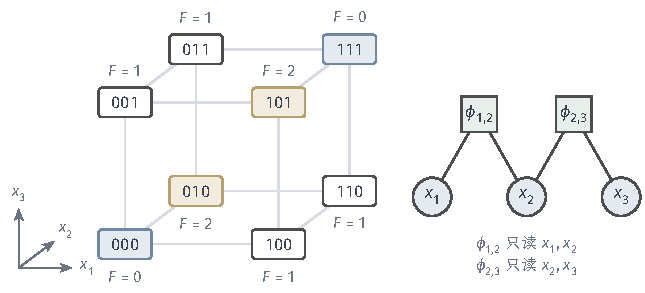
\includegraphics[width=109.269mm]{figures/01-basic-mathematics/04-graphs/tikz/c5-configuration-scopes/figure.pdf}
  \caption{配置空间与局部作用域。左：三个二值变量的$8$种配置排在立方体的顶点上，顶点旁的数是总成本$F=\phi_{1,2}+\phi_{2,3}$，其中相邻变量取值不同时成本为$1$；蓝色顶点成本为$0$，黄色顶点成本为$2$。右：圆点表示变量，方块表示局部函数，连线表示该函数读取的变量。每个局部函数只读取两个变量，但它们的和仍然对全部$8$种配置给出成本。}
  \label{fig:graph-dp-configuration-scopes}
\end{figure}

把这个例子一般化，设有一组局部项，用下标$a\in A$区分。每一项$\phi_a$只读取下标集合$S_a\subseteq V$中的变量，总成本为
\begin{equation}
F(\bm x)=\sum_{a\in A}\phi_a(\bm x_{S_a}),\qquad \bm x\in\mathcal X .
\label{eq:graph-dp-local-sum}
\end{equation}
这里的$\phi_a$称为\term{局部函数}（local function），也常称为\term{因子}（factor）；它读取的下标集合$S_a$称为$\phi_a$的\term{作用域}（scope）。“局部”限定的是读取范围：$\phi_a$精确地给出$\bm x_{S_a}$每种取值的成本，并不是对某个整体函数的近似；作用域也不限于两个变量，三元、四元的局部函数同样允许。一元项$\phi_i(x_i)$是作用域为$\{i\}$的特例。

局部函数的取值允许为$+\infty$，用来表示禁止的组合。例如设备$1,2$不能同时打开时，可以令$\phi_{1,2}(1,1)=+\infty$。约定$+\infty$加任何有限数或$+\infty$仍得$+\infty$，于是只要某一项禁止，整个配置的总成本就是$+\infty$。总成本有限的配置称为\term{可行配置}。这样，同一个式~\eqref{eq:graph-dp-local-sum}既表达偏好，也表达约束；求最小值时还要同时回答是否存在可行配置：最小值为$+\infty$，就说明所有配置都被某项禁止。

式~\eqref{eq:graph-dp-local-sum}是问题给出的分解，不是自动成立的性质。任意函数$F$都可以写成作用域为$V$的单个“局部”函数，但这时局部函数表就有$|\mathcal X|$项，与直接枚举没有区别。本章始终假定分解已经由问题给出，并且各作用域都较小；从一个任意给定的整体函数中寻找小作用域分解，是另一个问题。

\subsection{依赖图与因子图}

只有成对局部项时，可以用一个图记录哪些变量出现在同一项里：以变量为顶点，两个变量出现在同一个成对项中就连一条边。三台设备的例子得到路径$1-2-3$。这样的图记录的是函数的依赖关系，不是变量的取值本身；称“依赖结构是一条链”或“是一棵树”，指的就是这个图是路径或树。

三元及更高阶的局部项无法用一条边表示。这时把变量和局部函数分成两类节点：每个变量一个圆形节点，每个局部函数一个方形节点；变量属于某个局部函数的作用域时，在两者之间连边。这样得到的二部图称为\term{因子图}（factor graph）。因子图保留了每个局部函数的身份：两个不同的局部函数即使作用域相同，也是两个不同的方形节点。图~\ref{fig:graph-dp-configuration-scopes}右侧就是三台设备例子的因子图。

\paragraph{三种表示的对照}
考虑四个二值变量和两个三元局部函数，作用域分别为$S_A=\{1,2,3\}$和$S_B=\{2,3,4\}$。除因子图外，还有两种常用的结构表示。一种不保留函数节点，把每个作用域内的变量两两连边，得到的图称为\term{原始关系图}（primal graph），简称原始图。这里原始图有边$\{1,2\},\allowbreak\{1,3\},\allowbreak\{2,3\},\allowbreak\{2,4\},\allowbreak\{3,4\}$，唯独缺少$\{1,4\}$，因为变量$1$和$4$从不出现在同一个局部函数中。另一种允许一条“边”包含任意多个顶点：每个作用域记为一条\term{超边}（hyperedge），由此得到\term{超图}（hypergraph）。这里超图有两条超边$\{1,2,3\}$和$\{2,3,4\}$。图~\ref{fig:graph-dp-three-representations}并排画出了三种表示。

\begin{figure}[!htb]
  \centering
  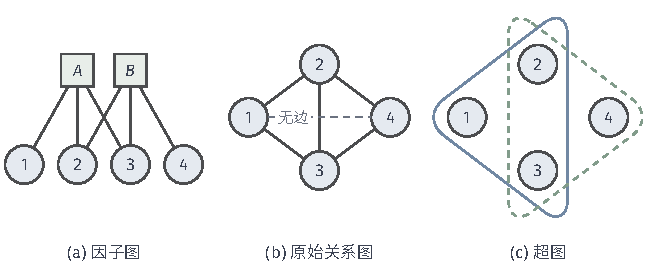
\includegraphics[width=111.936mm]{figures/01-basic-mathematics/04-graphs/tikz/c5-three-representations/figure.pdf}
  \caption{作用域$\{1,2,3\}$与$\{2,3,4\}$的三种结构表示。左：因子图，方块$A$、$B$是两个局部函数，连线表示读取关系。中：原始关系图，把每个作用域内的变量两两相连，只缺边$\{1,4\}$。右：超图，蓝色实线与绿色虚线围出的区域各是一条超边。若把两个三元函数换成五条边上的五个成对函数，原始图完全相同，而因子图和超图都会改变。}
  \label{fig:graph-dp-three-representations}
\end{figure}

原始图丢失了作用域的分组。若把$\phi_A,\phi_B$换成定义在五条边上的五个成对局部函数，原始图不变，因子图和超图却不同。更重要的是，相同的两两连接不能恢复函数表。设$\phi_A(x_1,x_2,x_3)$在$x_1+x_2+x_3$为偶数时取$0$、为奇数时取$+\infty$，$\phi_B$对$x_2+x_3+x_4$作同样的规定。$\phi_A$允许的取值恰为$(0,0,0),(0,1,1),(1,0,1),(1,1,0)$，其中任意两个变量的四种取值组合都出现过。因此，若只保留“每对变量允许哪些取值”的成对规则，这些规则什么也不禁止，$16$种配置都会被放行；而原问题中$x_2,x_3$确定后$x_1,x_4$都被唯一确定，只有$4$种可行配置。

超图保住了作用域的分组，但和原始图一样不保存局部函数的数值；因子图保住了函数身份，但仍需另外存储每个函数的取值表。后面的树分解以原始图为结构依据，因为原始图上的边已经足以说明哪些变量必须同时出现；计算时则始终使用完整的局部函数，不把它们拆成成对规则。
